In the dynamic landscape of distributed computing, the exponential growth in traffic demands within data centers and high-performance computing systems has been distinctive, fueled by a deluge of data-intensive workloads. This trend is prominently exemplified by the rapid expansion of machine learning, big data analytics, and most notably, deep learning (DL)\textendash driven artificial intelligence (AI) applications. The recent advent of large language models, which has revolutionized natural language processing and creative content generation, is propelling the broad adoption of ever-larger DL models and datasets, marking a significant milestone toward the era of data ubiquity. The continued scaling of these applications has pushed the limits of computational hardware, notably via increased parallelism and specialization. Yet, this rapid progress has outpaced the evolution of the underlying communication infrastructure, rendering chip-to-chip data movement a formidable barrier impeding performance and energy efficiency. This communication bottleneck has become the grand challenge to the quest of upscaling the computing systems toward exascale.

My research endeavors to find \textbf{transformative connectivity solutions}, maximally harnessing the potential of integrated silicon photonics (SiPh). In this pursuit, I have devised a dual-thrust research agenda for my independent career. The first thrust focuses on \textbf{reconfigurable system connectivity}. It aims to develop optical interconnects that not only provide unprecedented bandwidth but also adapt in real-time to the ever-evolving demands of emerging applications. The second thrust looks into \textbf{innovative system architectures}. It targets redefining chip-to-chip communication with groundbreaking optical I/O technologies, thereby pioneering new computational paradigms and interconnect functionalities. The synergy of these thrusts introduces unique design challenges, which I am equipped to tackle with my interdisciplinary research experience, ensuring the readiness of essential design tools and methodologies for these advanced connectivity solutions.

My research agenda is situated at the system level, squarely fitting into the interdisciplinary nexus of \appArea{} that bridges \appCollab{}. I look forward to the possibility of collaborating with the esteemed colleagues in the \appDept{} at the \appSchool{} to confront the grand challenge of data movement in future computing infrastructures across the full system stack.

\section{Research Accomplishments and Skills}
My doctoral and postdoctoral work have established a solid foundation for my anticipated research and equipped me with the skills necessary to address the upcoming research challenges. I was among the first to integrate accurate compact models and simulation methodologies of silicon photonic devices into widely used electronic design automation (EDA) platforms like Cadence Virtuoso~\cite{wuCompactModelingCircuitlevel2017,zhangCompactModelingSilicon2017}. This integration is crucial for the accurate co-simulation of electronic and photonic circuits, enabling the efficient development of complex photonic integrated circuits (PICs) with reliable performance estimation. My expertise in process variation characterization, mitigation, and tolerance~\cite{wangCharacterizationApplicationsSpatial2020,wangEnergyEfficiencyYield2021,wangDispersionEngineeredFabricationRobustSOI2023} ensures the robustness and energy efficiency of fabricated designs. This is particularly important for advanced technologies that often rely on emerging fabrication processes and require post-fabrication tuning.

These design enabling techniques were effectively utilized in creating two generations of SiPh transceiver chips, which incorporate a scalable link architecture for unprecedented channel parallelism and deliver a chip I/O bandwidth of over 16 Tbps with energy consumption below 1\,pJ/b~\cite{wangScalableArchitectureSubpJ2023,wangCICC2024}. Fabricated in partnership with AIM Photonics through two full-wafer runs, each chip featured a \textasciitilde{}70\,mm$^\text{2}$ footprint integrated with over 2,000 microresonators. The design process was fully automated using a scripted layout approach, demonstrating exceptional design efficiency in addition to the technological advancement that these chips represent.

System level \cite{wangTaskMappingAssistedLaser2019,wangTrafficAdaptivePowerReconfiguration2021,brianJOCN}

\section{Research Vision and Agenda}
Some leading sentences here.
\subsection{Thrust 1: Reconfigurable System Connectivity}
The need for high-bandwidth and energy-efficient connectivity is ubiquitous across all levels of network hierarchies. That, combined with growing concerns over traffic heterogeneity and dynamics, motivates the pursuit of

\subsection{Thrust 2: Innovative System Architectures}


\section{Research Collaborations and Initiatives}

\begin{figure}[!ht]%
    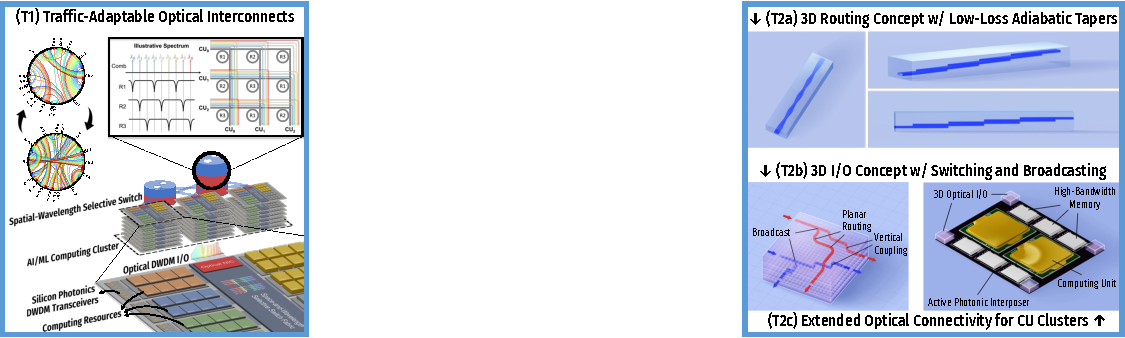
\includegraphics[width=\linewidth]{../../fig/research.pdf}
    \caption{Cross-level design enablement and optimization techniques serving as research foundation.}
    \label{fig:research}
\end{figure}

My interdisciplinary research vision is positioned at the intersection of electronics/photonics, devices/systems, and design/applications. It necessitates a collaborative synthesis across various sub-disciplines, which I conceptualize along two orthogonal dimensions, as depicted in Fig.~\ref{fig:research}. The comprehensive skill set acquired through my doctoral and postdoctoral experiences has allowed me to integrate design methodologies and optimization techniques in both vertical and horizontal facets, thereby laying a solid groundwork for the research agenda that I propose. The expertise and insights gained from these endeavors will seamlessly inform and underpin the trio of research thrusts that I will elaborate as following.

\section{Thrust 1: Traffic-Adaptable Optical Interconnects}

With the advent of augmented reality (AR), virtual reality (VR), and Metaverse applications, distributed machine learning frameworks are seeing an increase in data privacy concerns that were previously confined to sectors with sensitive information, such as banking and healthcare. These sectors typically handle smaller volumes of data with more flexible latency requirements. In response, decentralized learning frameworks like federated learning have been preferred, as they allow the exchange of model parameters over raw data. Yet, certain applications still prioritize data parallelism to meet stringent requirements on model accuracy. Consequently, the data landscape in distributed computing is evolving toward not only larger volumes but also greater heterogeneity. This shift necessitates the next-generation of optical interconnects to provide traffic-adaptable runtime reconfiguration capabilities, in addition to high bandwidth capacities, to accommodate these evolving demands.

This research direction will leverage the pioneering work on integrated silicon photonics chip I/O from my postdoctoral studies\cite{wangScalableArchitectureSubpJ2023}, which achieved ultra high-bandwidth and low-energy transmission through a scalable dense wavelength division multiplexing (DWDM) link architecture. Additionally, it will build upon preliminary investigations into bandwidth reconfiguration within distributed deep learning environments, where previously, traffic patterns exhibited less temporal variations\cite{brianJOCN}.

The successful advancement of this research thrust will involve the following critical tasks:
\begin{enumerate}[nosep]
    \item Develop and incorporate a runtime reconfiguration module within the DWDM link architecture, facilitating dynamic bandwidth allocation that adjusts to varying traffic patterns and specific application needs. A preliminary off-chip prototype that divides wavelength channels between two ports has shown promise and is undergoing publication review, with an on-chip version already sent to AIM Photonics for fabrication and slated for testing in April 2024. Future iterations will focus on expanding port numbers, fine-tuning splitting ratios, accelerating reconfiguration times, and enabling channel reassignment.
    \item Profile the traffic patterns of a selection of key distributed computing applications to shape the development of runtime reconfiguration strategies.
    \item Conduct system-level simulations to assess the energy and performance impacts of the proposed runtime reconfiguration strategies.
    \item Implement and test the envisioned interconnect architecture and reconfiguration strategies on a hardware testbed, using real production network traces to validate the approach.
\end{enumerate}
By addressing the critical need for adaptive, high-performance optical interconnects that can keep pace with the ever-increasing demands of modern computing applications, this research thrust has the potential to reshape the landscape of future distributed computing infrastructures with tangible improvements in efficiency and versatility.

\begin{figure}[!ht]%
    \includegraphics[width=\linewidth]{../../fig/stair.png}
    \caption{Conceptual rendering of compact 3D waveguide routing enabled by multiple layers of low-loss adiabatic tapers.}
    \label{fig:stair}
\end{figure}
\begin{figure}[!ht]%
    \includegraphics[width=\linewidth]{../../fig/cube.png}
    \caption{Conceptual rendering of a 3D optical I/O featuring switching and broadcasting capabilities for flexible die-to-die connectivity.}
    \label{fig:cube}
\end{figure}

\section{Thrust 2: 3D Optoelectronic Architectures}

State-of-the-art accelerator systems, composed of clusters of computing units (CUs), are confronting a ``memory wall'' caused by the significant disparity between the bandwidth for intra- and inter-cluster communications. The option to expand the number of on-chip high-bandwidth memory (HBM) stacks is becoming less viable as the bandwidth capacity of electronic interposers nears saturation. Traditional approaches using optical fibers for interconnecting memory pools are impractical for densely arranged CU clusters due to the size and pitch limitations of fiber arrays. Nonetheless, the emerging concept of 3D optical I/Os, which facilitate dense waveguide routing in multiple layers, could unlock new possibilities for scaling up CU clusters with optical connectivity achieved directly through waveguides. Having contributed to the preparation for the concept's showcase at the 2023 DARPA ERI Summit, I am inspired to pursue this avant-garde research thrust, which has the potential to pioneer a novel computing architecture through a deeply integrated electronic-photonic synergy. I look forward to exploring several key research topics, in collaboration with field experts, including:
\begin{enumerate}[nosep]
    \item The device-level design and optimization of multi-layered 3D optical I/O modules for high-density, low-loss, and compact optical interfaces, incorporating innovative coupling mechanisms.
    \item The architectural investigation of optically interconnected accelerator systems featuring dense, fiber-less connectivity to delineate the optimal configuration for system-level designs.
    \item The pursuit of novel functionalities for on-chip silicon photonics, leveraging enhanced density and routing capabilities to perform computational tasks, extending beyond traditional data communication roles.
\end{enumerate}
The fruition of this research direction promises not just to scale accelerator systems in alignment with the computational demands of the future, but also to broaden the scope for on-chip optical interconnects to assume a more dynamic and integral role in computing architectures.

\begin{figure}[!ht]%
    \includegraphics[width=\linewidth]{../../fig/new_arch.png}
    \caption{Conceptual rendering of densely interconnected computing units featuring fiber-less optical connectivity.}
    \label{fig:new_arch}
\end{figure}

\section{Thrust 3: Design Automation for Future Integrated Photonics}
Successfully navigating the design and optimization intricacies presented by the proposed research thrusts is crucial for actualizing the advanced connectivity solutions I envision. The anticipated challenges include:
\begin{enumerate}[nosep]
    \item Developing efficient yet accurate modeling and simulation methodologies for the envisioned connectivity solutions at device, circuit, and system levels, democratizing the design process and enabling rapid prototyping and design optimization.
    \item Characterizing and mitigating process variations, along with creating designs that are robust against fabrication inconsistencies, especially crucial for the experimental processes involved in the second research thrust.
    \item Creating novel design enablement technologies that exploit machine learning and artificial intelligence to expand the design capabilities for future integrated photonics.
\end{enumerate}
With the cross-disciplinary design ecosystem that I have cultivated during my academic journey\cite{wangDispersionEngineeredFabricationRobustSOI2023}\cite{wangCharacterizationApplicationsSpatial2020}\cite{wangEnergyEfficiencyYield2021}, I am poised to leverage my expertise to forge a comprehensive design automation framework for the next generation of integrated silicon photonics interconnect systems.


\section{Research Collaborations and Initiatives}
My experience has been deeply rooted in multidisciplinary collaboration, a skill I mastered during my postdoctoral training at Columbia University, where I spearheaded research initiatives within our group, guided by my supervisor, and fueled by DARPA and SRC funding. These initiatives necessitated seamless teamwork with colleagues from academia, industry, and governmental bodies. Additionally, I have a proven track record of supporting my advisor in fundraising endeavors, notably contributing to the writing and visual elements of a successful \$35M SRC JUMP 2.0 grant application. My role also extended to compiling regular reports and presenting at quarterly reviews to meet the obligations of our funded projects.

I am eager to bring my expertise and enthusiasm to your esteemed university, where I look forward to collaborating with a community that shares my dedication to innovation and to making a meaningful impact on the future of technology.

